\chapter{Signal selection}

\label{ch:ana-sig}

\par Signal selection is a process to select target events with multiple filtering criteria based on the event signature. In this article, in order to obtain a high signal over background efficiencies, the physics object level selection is applied first, then, signal regions are designed. Moreover, control regions are also defined to constrain the background contribution.

\section{Physics objects definition}
\label{sec:ana-sig:physobj}

\par As mentioned previously, leptons, jets and missing transverse momentum are the variables that are helpful to increase signal selection efficiencies.

\subsection{Leptons}

\begin{itemize}
    \item \textbf{Electrons}: As mentioned in Section~\ref{sec:el}, electrons can be dentified using various likelihood-base criteria, for example, shower profile selections, track quality, and high threshold TRT hits. The electron identification criteria that used in this analysis are listed In Table~\ref{tab:c7:physobj:ele}.
    \item \textbf{Muons}: Muons are reconstructed with a combined information from inner tracker and muon spectrometer. Moreover, two different working points are applied in this analysis for muon identification. A loose criteria is applied as baseline muon selection to obtain larger acceptance, while medium working point is used in signal selection for higher purity. More details are listed in Table~\ref{tab:c7:physobj:muo}.
    \item \textbf{$\tau$-Leptons}: As decribed in Section~\ref{sec:taus}, $\tau$-lepton is reconstructed using inner tracker and calorimeter. Since the $\tau$-lepton is vetoed in both signal and control regions, a loose $\tau$-lepton working point is enough for this analysis. More information can be found in Table~\ref{tab:c7:physobj:tau}.
\end{itemize}

\begin{table}[ht]
    \caption{Electron selection criteria.}
    \label{tab:c7:physobj:ele}
    \centering
    \begin{tabular}{|c|c|}
        \hline
        Feature & Criterion \\
        \hline
        \hline
        Pseudorapidity range & \(|\eta| < 2.47\) \\
        \hline
        Transverse momentum & \pt $> 7GeV$ \\
        \hline
        Track to vertex association & \(|d_{0}^{\text{BL}}(\sigma)| < 5\)\\ & \(|\Delta z_{0}^{\text{BL}} \sin{\theta}| < 0.5mm\) \\
        \hline
        Identification & \texttt{FCLoose} \\
        \hline
        Isolation & \texttt{LooseTrackOnly / FCHighPtCaloOnly} \\
        \hline
    \end{tabular}
\end{table}

\begin{table}[ht]
    \caption{Muon selection criteria.}
    \label{tab:c7:physobj:muo}
    \centering
    \begin{tabular}[ht]{|c|c|c|}
        \hline
        Feature & Baseline criterion & Signal criterion \\
        \hline
        \hline
        Selection working point & \texttt{Loose} & \texttt{Medium} \\
        \hline
        Isolation working point & \texttt{FCLoose} &  \texttt{FCTightTrackOnly} \\
        \hline
        Momentum calibration & Sagitta correction & Sagitta correction \\
        \hline
        \pt cut & 7GeV & 7GeV \\ 
        \(|\eta|\) cut & \(< 2.7\) & \(< 2.5\) \\
        \hline
        \(d_{0}\) significance cut & 3 & 3 \\
        \hline
        \(z_{0}\) cut & 0.5mm & 0.5mm \\
        \hline
    \end{tabular}
\end{table}

\begin{table}[ht]
    \caption{Tau selection criteria.}
    \label{tab:c7:physobj:tau}
    \centering
    \begin{tabular}{|c|c|}
        \hline
        Feature & Criterion \\
        \hline
        \hline
        Pseudorapidity range & \(|\eta| < 2.5\) \\
        \hline
        Track selection & 1 or 3 tracks \\
        \hline
        Charge & \(|Q| = 1\) \\
        \hline
        Tau energy scale & \texttt{MVA TES} \\
        \hline
        Transverse momentum & \pt $> 20GeV$ \\
        \hline
        Jet rejection & BDT-based (\texttt{Loose}) \\
        \hline
        Electron rejection & BDT-based \\
        \hline
        Muon rejection & \specialcell{Via overlap removal in \(\Delta R < 0.2\) and \pt $> 2GeV$.\\ Muons must not be Calo-tagged} \\
        \hline
    \end{tabular}
\end{table}

\subsection{Jets}

\begin{itemize}
    \item \textbf{Small-radius jets}: As mentioned in Section~\ref{sec:jets}, the small-radius jets can be divided into two categories: central jets and forward jets. In this analysis, only the central jets are used to reconstruct Higgs boson, while both central and forward jets are involved in \met calculation. More informtion about small-radius jets identification can be found in Table~\ref{tab:c7:physobj:srjets}.
    \item \textbf{Large-radius jets}: The large-radius jets are recontructed with large cone size (R=1.0). These large cone size jets are used to reconstruct the boosted Higgs boson. More details are listed in Table~\ref{tab:c7:physobj:lrjets}.
    \item \textbf{Variable-radius track jets}: The variable-radius track jets are reconstructed from inner tracker using anti-$k_{t}$ algorithm. The jet radius is dependent on the jet \pt: $R=\frac{30GeV}{p_{T}}$. The variable-radius track jets provide a better acceptance when reconstructing boosted Higgson boson in this analysis.
    \item \textbf{b-jets}: The b-tagging is a technology to identify the b-jets, which is applied on central jets to reconstruct the resolved Higgs boson. More detailed information can be found in Table~\ref{tab:c7:physobj:bjets}.
\end{itemize}

\begin{table}[ht]
    \caption{Small-\(R\) jet reconstruction criteria.}
    \label{tab:c7:physobj:srjets}
    \centering
    \begin{tabular}{|c|c|}
        \hline
        Feature & Criterion \\
        \hline
        \hline
        Algorithm & Anti-$k_{t}$ \\
        \hline
        \(R\)-parameter & 0.4 \\
        \hline
        Input constituent & PFlow \\
        \hline
        \texttt{CalibArea} tag & 00-04-82 \\
        \hline
        Calibration configuration & \specialcell{\texttt{JES\_MC16Recommendation\_}\\\texttt{Consolidated\_EMTopo\_Apr2019\_Rel21.config}} \\
        \hline
        Calibration sequence (Data) & \texttt{JetArea\_Residual\_EtaJES\_GSC\_Insitu} \\
        \hline
        Calibration sequence (MC) & \texttt{JetArea\_Residual\_EtaJES\_GSC} \\
        \hline
        Jet cleaning & \texttt{TightBad} \\
        \hline
        \pt & \(> 20GeV\) (central) / \(> 30GeV\) (forward) \\
        \hline
        \(|\eta|\) & \(< 2.5\) (central) /  \(2.5 < |\eta| < 4.5 \) (forward) \\
        \hline
        JVT & \specialcell{\texttt{Medium} working point,\\applied only to central jets with \pt $< 120GeV$} \\
        \hline
    \end{tabular}
\end{table}
    
\begin{table}[ht]
    \caption{Large-\(R\) jet reconstruction criteria.}
    \label{tab:c7:physobj:lrjets}
    \centering
    \begin{tabular}{|c|c|}
        \hline
        Feature & Criterion \\
        \hline
        \hline
        Algorithm & Anti-$k_{t}$ \\
        \hline
        R-parameter & 1.0 \\
        \hline
        Input constituent & \texttt{LCTopo} \\
        \hline
        Grooming algorithm & Trimming \\
        \hline
        Subjet \pt fraction for trimming & 0.05 \\
        \hline
        \(R_{\text{trim}}\) & 0.2 \\
        \hline
        \texttt{CalibArea} tag & 00-04-82 \\
        \hline
        Calibration configuration (Data) & \specialcell{\texttt{JES\_MC16recommendation\_FatJet}\\\texttt{\_Trimmed\_JMS\_comb\_3April2019.config}} \\
        \hline
        Calibration configuration (MC) & \specialcell{\texttt{JES\_MC16recommendation\_FatJet}\_\\\texttt{Trimmed\_JMS\_comb\_17Oct2018.config}} \\
        \hline
        Calibration sequence (Data) & \texttt{EtaJES\_JMS\_Insitu} \\
        \hline
        Calibration sequence (MC) & \texttt{EtaJES\_JMS} \\
        \hline
        \pt & \(> 200GeV\) \\
        \hline
        \(|\eta|\) & \(< 2\) \\
        \hline
    \end{tabular}
\end{table}

\begin{table}[ht]
    \caption{b-jets selection criteria.}
    \label{tab:c7:physobj:bjets}
    \centering
    \begin{tabular}{|c|c|}
        \hline
        Feature & Criterion \\
        \hline
        \hline
        Jet collection & \texttt{AntiKt4EMPFlow / AntiKtVR30Rmax4Rmin02} \\
        \hline
        Algorithm & \texttt{DL1} \\
        \hline
        Operating point & Eff = 77 \\
        \hline
        CDI & \texttt{2017-21-13TeV-MC16-CDI-2019-07-30\_v1} \\
        \hline
    \end{tabular}
\end{table}
  
\subsection{Missing transverse momentum}

\par As described in Section~\ref{sec:met}, the missing transverse momentum (\met) is defined as the magnitude of missing transverse momentum vector, which is calculated by all well-reconstructed physics object, like electron, muon and jets. More information about \met~reconstruction is listed in Table~\ref{tab:c7:physobj:met}.

\begin{table}[ht]
    \caption{\met reconstruction criteria.}
    \label{tab:c7:physobj:met}
    \centering
    \begin{tabular}{|c|c|}
        \hline
        Parameter & Value \\
        \hline
        \hline
        Algorithm & Calo-based \\
        \hline
        Soft term & Track-based (TST) \\
        \hline
        \met operating point & \texttt{Tight} \\
        \hline
    \end{tabular}
\end{table}

\section{Signal regions}
\label{sec:ana-sig:sigreg}
\par Signal regions are a set of phrase spaces that is defined by a combination of selection conditions for signal selection. In this analysis, the most important signature is Higgs boson, which have different signatures under different energy scales. Therefore, Resolved region and Merged region are designed as sub signal regions to probe signals effectively under different Higgs boson momentum signatures.

\subsection{Common event selection}
\par Several common event selection criteria are applied for both resolved and merged regions as a baseline selection.
\begin{itemize}
    \item \textbf{Event cleaning}: Event cleaning is a process to apply a set of filters to veto the corrupted events. In this analysis, LAr noise burst, tile corruption, SCT recovery procedure and incomplete events are applied as the event cleaning filters. More information can be found in \cite{c8-evt-cleaning}.
    \item \textbf{Loose jet Veto}: In analysis, the reconstructed jets can be a fake jet from noise, collision background, etc.. TightBadJet criteria, provided by Jet/\met group, is applied in this analysis to veto events that contain the fake jets.
    \item \textbf{\met~selection}: In signal regions, a constrain \met $>150GeV$ is applied. In control region, the lepton momentum is also treated as part of missing transverse momentum and same \met cut is applied.
    \item \textbf{Light lepton and $\tau$-lepton veto}: Events that contain a electron, muon or $\tau$-lepton, as defined in Section~\ref{sec:ana-sig:physobj}, are rejected.
    \item \textbf{Extended $\tau$-lepton veto}: An extended $\tau$ veto is applied in case of $\tau$-lepton failed to be identified. A hadronically decayed $\tau$ can be viewed as a jet. Therefore, a jet is considered as a $\tau$ candidate if it fullfills two conditions: (1) The track multiplicity in the jet cone is between 1 to 4. (2) The angular separation between the jet and \met is $\Delta \phi \leq 22.5^\circ$. The cut on the track multiplicity in the jet cone makes sure that the hadronic decay products in the jet are compatible with the $\tau$-lepton decay products, namely with charged pions. The tracks considered are associated with the primary vertex and have a \pt greater than 1 GeV. The cut on the angular separation between jet and \met makes sure that the $\tau$-candidate comes from a W boson.
    \item \textbf{$\min_{j \in \{1,2,3\}}\Delta\phi(E_{\mathrm{T}}^{\mathrm{miss}},j)$}: QCD multijet events can be generated by jet energy mis-measurement. In case of fake \met, the \met will generally point to the direction of leading jets. Therefore, an angular cut between \met and leading jets is applied to veto these events.
\end{itemize}

\par After these baseline selection, signal region needed to be analyzed on different sub regions based on Higgs boson signature. In the target model, the sum of \met vector and Higgs boson momentum vector should be zero based on momentum conservation. Therefore, one can apply a single cut on \met to separate events with resolved or merged Higgs boson. In this analysis, the cut \met$<500GeV$~is defined as resolved region while \met$>500GeV$ is merged region. The Higgs boson identification, which will be demonstrate in the rest of this section, is different in these two signal regions.
\par Moreover, there is one additional condition to select events with at lease one b-jets. The b-tagging is applied on all small-radius central jets in resolved region, while only on two leading track jets that associated to large-radius jet in merged region.

\subsection{Resolved region}

\par In resolved region, the Higgs boson momentum is relative low. Therefore, the Higgs boson decay products, two b-jets, can be resolved into two separate jets. To reconstruct the Higgs boson, a set of jet candidates needed to be selected first. There are two categories in the Higgs boson jets candidate set: (1) b-tagged jets, (2) central non b-tagged jets. The jets are ordered in decreasing transverse momentum within each category. The first two out of this set of jets (referred as j1 and j2 below) are used to reconstruct Higgs boson candidate, which referred as $H_{reco}$.

\par There are several criteria to select Higgs boson in resolved channel:

\begin{itemize}
    \item \textbf{\pt of $H_{reco}$}: \pt of $H_{reco}$ is expected to increase with \met. Therefore, a cut \pt$(H_{reco})>100GeV$ is applied when \met $<350GeV$, while \pt$(H_{reco})>300GeV$ when $350GeV<$\met$<500GeV$.
    \item \textbf{$m_{jj}$}: A window cut on the mass of reconstructed Higgs boson is helpful to identify the Higgs boson. The mass of reconstructed Higgs boson can be calculated from the invariant mass of jets pair ($m_{jj}$) that form $H_{reco}$. A window cut $50GeV<m_{jj}<280GeV$ is applied in this analysis. 
    \item \textbf{$m_{T}^{b}$}: In resolved region, the major background is top quark pair production. $m_{T}^{b}$ is introduced to reject these background events. The $m_{T}^{b}$ is defined as: $m_{T}^{b}=\sqrt{2p_{T}^{b}E_{T}^{miss}(1-cos\Delta\phi(\vec{p}_{T}, \vec{E}_{T}^{miss}))}$. The $m_{T}^{b}$ is calculated on the b-jets that closest to and furtherest from \met. The closest b-jet $m_{T}^b$ is required to be greater than 170 GeV, while the furtherest cut is greater than 200 GeV.
\end{itemize}

\par In addition, it is possible that the measured \met of an event is due to a resolution fluctuation. Therefore, a \met significance cut $S>12$ is introduced to reject fake \met events.

\subsection{Merged region}

\par In merged region, the momentum of Higgs boson is relative high, and therefore, the products of this high energy Higgs boson are merged into one fat cone, which is reconstructed as a large-radius jet in detector.
\par Several criteria are applied on the large-radius to identify the Higgs boson in merged region:
\begin{itemize}
    \item \textbf{$m_{J}$}: The invariant mass of the large-radius jet is an expression of Higgs boson mass. A window cut $50GeV<m_{J}<270GeV$ is applied.
    \item \textbf{Variable-radius track jets association}: At least two variable-radius track jets needed to be associated to the large-radius jet.
\end{itemize}

\par As a summary of Section~\ref{sec:ana-sig:sigreg}, both resolved and merged signal regions are listed in Table~\ref{tab:c7:sigreg:summary}.

\begin{table}[h]
    \centering
	\begin{center}
        \begin{tabular}{cc}
            \hline
            \textbf{Resolved} & \textbf{Merged} \\
            \hline
            \hline
            \multicolumn{2}{c}{lowest unprescaled \met trigger} \\
            \hline
            \multicolumn{2}{c}{veto on baseline light leptons and $\tau$-leptons} \\
            \hline
            \multicolumn{2}{c}{extended $\tau$-veto} \\
            \hline
            \multicolumn{2}{c}{\met $>150GeV$} \\
            \hline
            \multicolumn{2}{c}{$\mindphi > 20^\circ$} \\
            \hline
            \met $< 500GeV$ & \met $> 500GeV$ \\
            \hline
            N(central small-R jets) $\geq 2$ & N(central large-R jets) $\geq 1$ \\
            \hline
            N($b$-tagged small-R jets) $\geq 1$ & N($b$-tagged associated track jets) $\geq 1$ \\
            \hline
            $S>12$ & --- \\
            \hline
            \pt$(jj) > 100GeV$ if \met $< 350GeV$ & --- \\
            \hline
            \pt$(jj) > 300GeV$ if \met $\geq 350GeV$ & --- \\
            \hline
            $\mtb{\min} > 170GeV$& --- \\
            \hline
            $\mtb{\max} > 200GeV$& --- \\
            \hline
            $50GeV < m_{jj} < 280GeV$ & $50GeV < m_{J} < 270GeV$ \\
            \hline
            b-tagging on small-radius jets & b-tagging on variable-radius track jets \\
            \hline
		\end{tabular}
	\end{center}
	\caption{Summary of the resolved and merged event selection applied in the 0-lepton channel. $\mathcal{S}$ denotes the object based \met significance.}
	\label{tab:c7:sigreg:summary}
\end{table}

\section{Control regions}
\label{sec:ana-sig:ctlreg}
\par Control regions are a set of phrase spaces that are orthogonal to signal regions. Control regions are designed to estimate the contribution of backgrounds in signal regions.

\subsection{1-lepton channel}
\par In the signal region the W+jets related background is mostly composed of events in which the $W$-boson decays leptonically. The $t\bar{t}$ background in the signal region originates almost only from semileptonic $t\bar{t}$ decays. Events with leptons can enter the signal region if the leptons fail to be identified or if they are outside the detector acceptance. The largest contribution comes from decays involving $\tau$-leptons, as shown in Figure~\ref{fig:ttbarDecayCat}. Figure~\ref{fig:ttbarDecayCatKinematic} shows the distribution of different kinematic variables for the dominant decay modes. From these it can be seen that shapes of the event variables agree well within the statistical uncertainties. Therefore the W+jets and $t\bar{t}$ backgrounds can be estimated using a 1-lepton control region, in which the lepton could have any flavor in principle.

\begin{figure}[h]
    \centering
    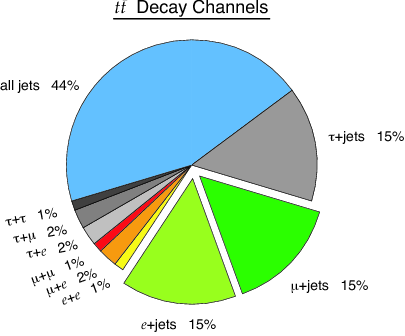
\includegraphics[width=0.9\textwidth]{chapters/c7/figures/ttbar-decay-modes.png}
    \caption{Decay categories for $t\bar{t}$ events in the signal region. The classification of the decay processes was performed by examining the truth particle information within the reconstructed signal region events. The three dominant decay modes are the semileptonic decays with either a light lepton, a leptonically or a hadronically decaying $\tau$-lepton.}
    \label{fig:ttbarDecayCat}
\end{figure}

\begin{figure}[h]
    \centering
	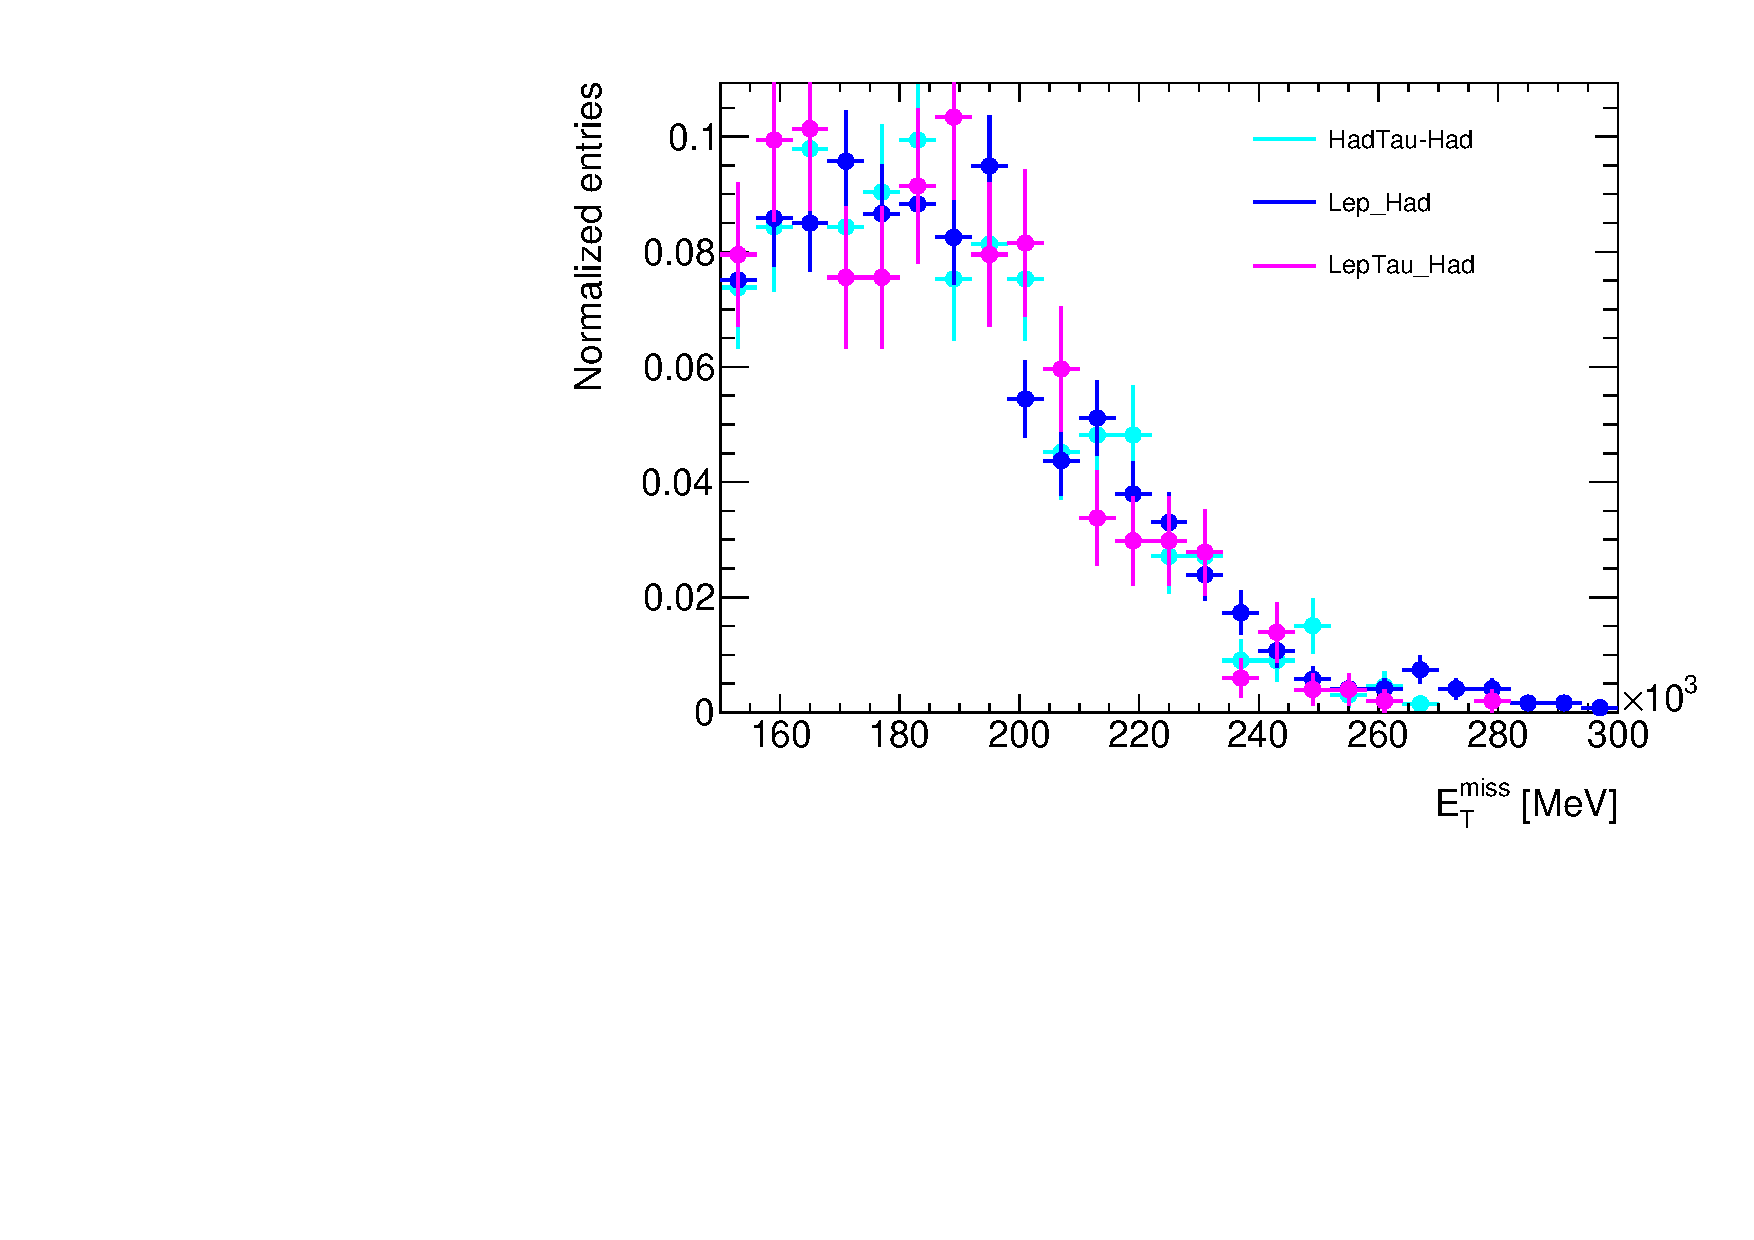
\includegraphics[width=0.45\textwidth]{chapters/c7/figures/ttbar_MetTST_met.pdf}
	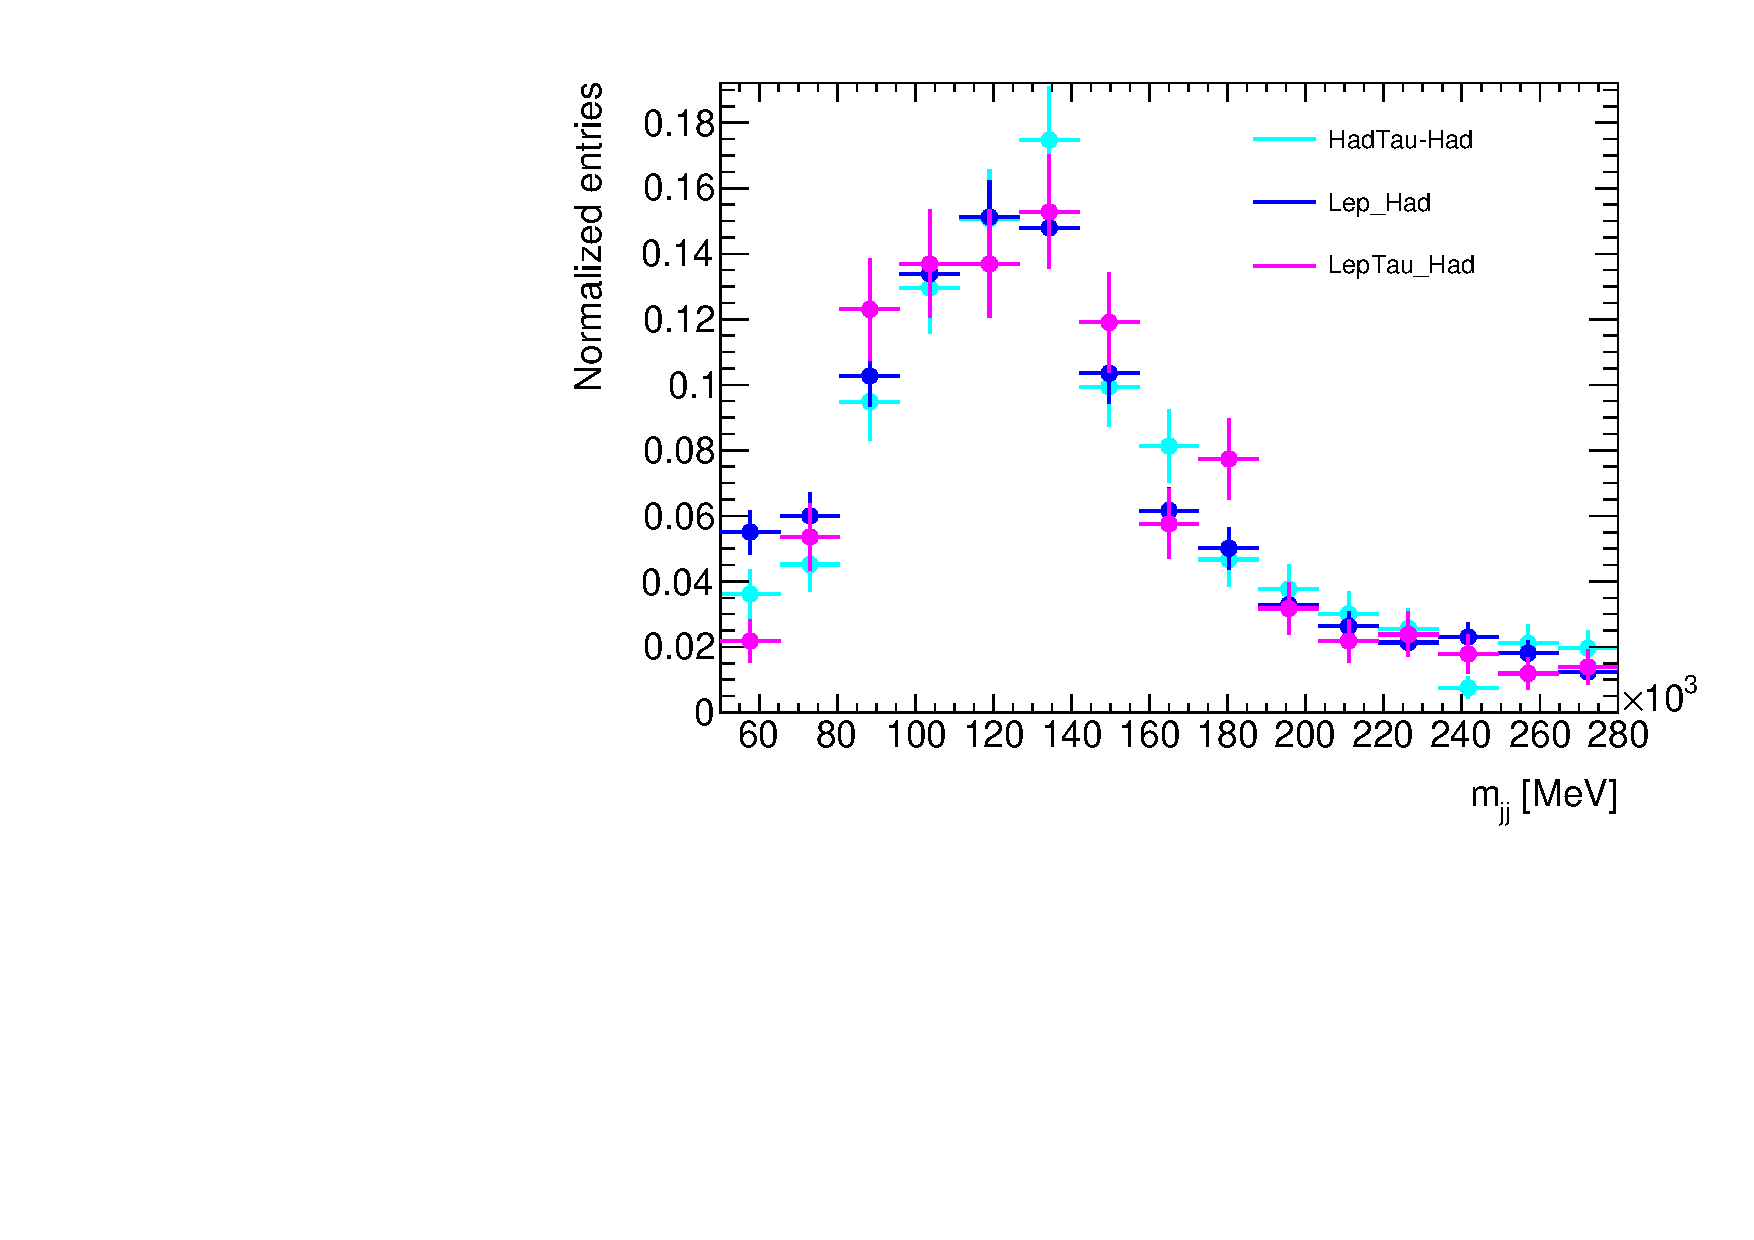
\includegraphics[width=0.45\textwidth]{chapters/c7/figures/ttbar_m_jj.pdf}
	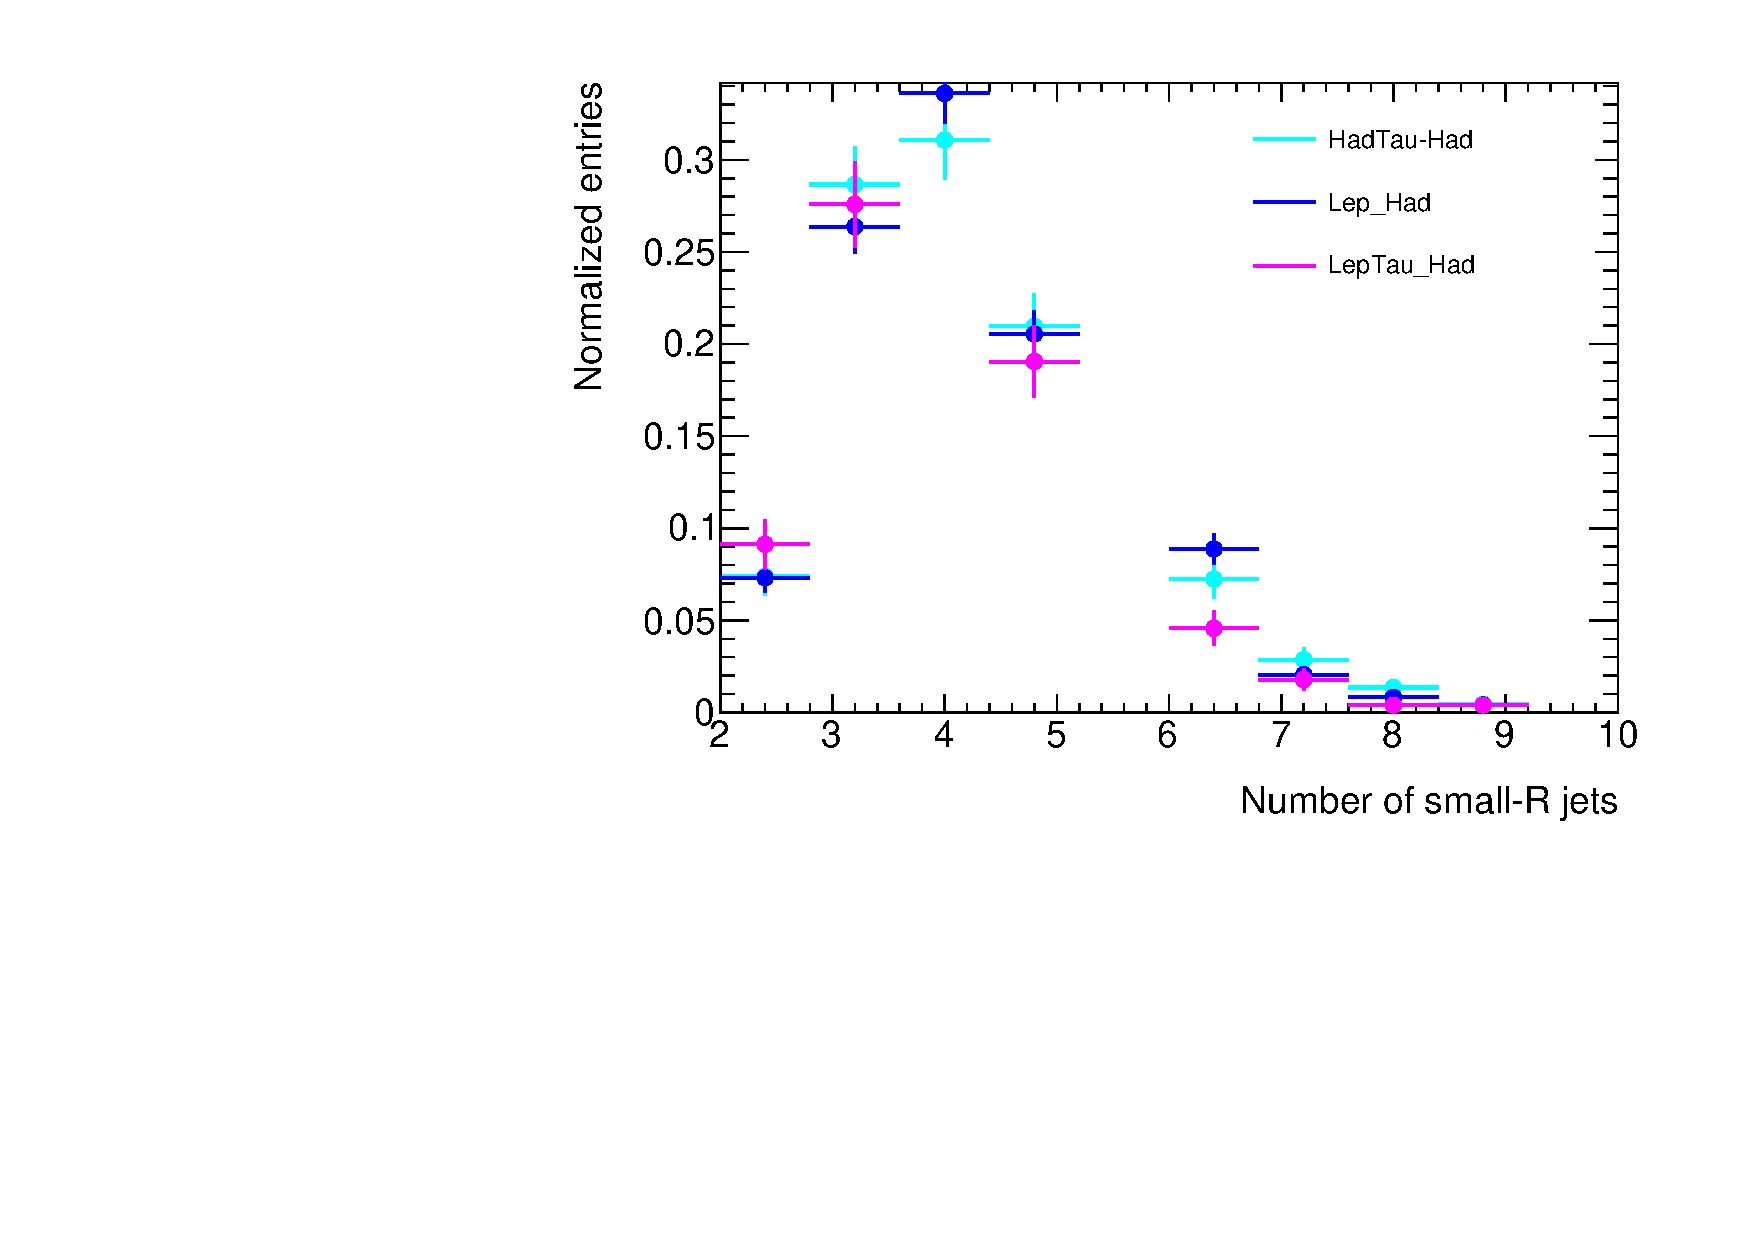
\includegraphics[width=0.45\textwidth]{chapters/c7/figures/ttbar_N_Jets04.pdf}		
	\caption{Normalised distributions of \met, the Higgs boson candidate mass and the number of small-radius jets for $t\bar{t}$ events. The distributions are shown separately for the three semileptonic decay modes, which are the dominant decays modes in the signal region. The shapes of the distributions agree well within the statistical uncertainties.}
	\label{fig:ttbarDecayCatKinematic}
\end{figure}

\par The 1-muon control region is chosen to constrain W+jets related background. Events in this control region is required to have exactly muon and no other baseline leptons.

\subsection{2-lepton channel}
\par A 2-lepton control region is used to estimate the Z+jets background. In the signal region the $Z(\to\nu\nu)+jets$ production leads to a significant amount of background events, which have the same decay topology as $Z(\to\ell\ell)+jets$, because the momentum of the $Z$ boson does not depend on its decay products. Hence the normalisation of $Z(\to\nu\nu)+jets$ events can be estimated with the help of a $Z(\to\ell\ell)+jets$ control region.

\par The 2-lepton control region is defined by selecting exactly two muons or two electrons. At least one of the lepton need to saitisfy the signal lepton criteria with enough \pt to pass the trigger. The signal muon is required to have \pt $>25GeV$, while signal electron is \pt $>27GeV$. The other lepton is not required to pass signal lepton selection to increase the acceptance. More over, since the two lepton is supposed to reconstruct Z boson, a mass window requirement is implemented to identify the Z mass peak: $|m_{Z}-m_{ll}|<10GeV$.
